\documentclass[xcolor=dvipsnames]{beamer}
\usepackage[T1]{fontenc}
\usepackage[utf8]{inputenc}
\usepackage[english,slovak]{babel}

\usepackage{amsmath}
\usepackage{amsthm}
\usetheme{Pittsburgh}
\useoutertheme{shadow}

\usepackage{graphicx}
\usepackage{caption}
\usepackage{subcaption}

\usepackage[]{algorithm2e}
\usepackage{listings}
 \setbeamercovered{transparent}
 \usepackage{cuted}
\usepackage[export]{adjustbox}
\usepackage{mathtools}

\usepackage{lipsum}
\usepackage{verbatim}
\usepackage{transparent}
\usepackage{framed}
\usepackage{xcolor}

\usepackage{multirow}
\usepackage{colortbl}
\usepackage{lmodern}

\usepackage{movie15}
\usepackage{verbatim}

\usepackage{hyperref}

\newcommand\Wider[2][3em]{%
\makebox[\linewidth][c]{%
  \begin{minipage}{\dimexpr\textwidth+#1\relax}
  \raggedright#2
  \end{minipage}%
  }%
}






\iffalse

\usetheme{Warsaw}

\setbeamercolor{normal text}{fg=white,bg=black!90}
\setbeamercolor{structure}{fg=white}

\setbeamercolor{alerted text}{fg=red!85!black}

\setbeamercolor{item projected}{use=item,fg=black,bg=item.fg!35}

\setbeamercolor*{palette primary}{use=structure,fg=structure.fg}
\setbeamercolor*{palette secondary}{use=structure,fg=structure.fg!95!black}
\setbeamercolor*{palette tertiary}{use=structure,fg=structure.fg!90!black}
\setbeamercolor*{palette quaternary}{use=structure,fg=structure.fg!95!black,bg=black!80}

\setbeamercolor*{framesubtitle}{fg=white}

\setbeamercolor*{block title}{parent=structure,bg=black!60}
\setbeamercolor*{block body}{fg=black,bg=black!10}
\setbeamercolor*{block title alerted}{parent=alerted text,bg=black!15}
\setbeamercolor*{block title example}{parent=example text,bg=black!15}

\fi



%-------------------------------------------------------------------------------------
\title{\color{white} \bf DQN}
\author{\color{white} Michal CHOVANEC, PhD}


%\setbeamertemplate{footline}[frame number]{}
\setbeamertemplate{navigation symbols}{}


\date[EURP]{}
\begin{document}

{
    \usebackgroundtemplate
    {
        \vbox to \paperheight{\vfil\hbox to \paperwidth{\hfil

        {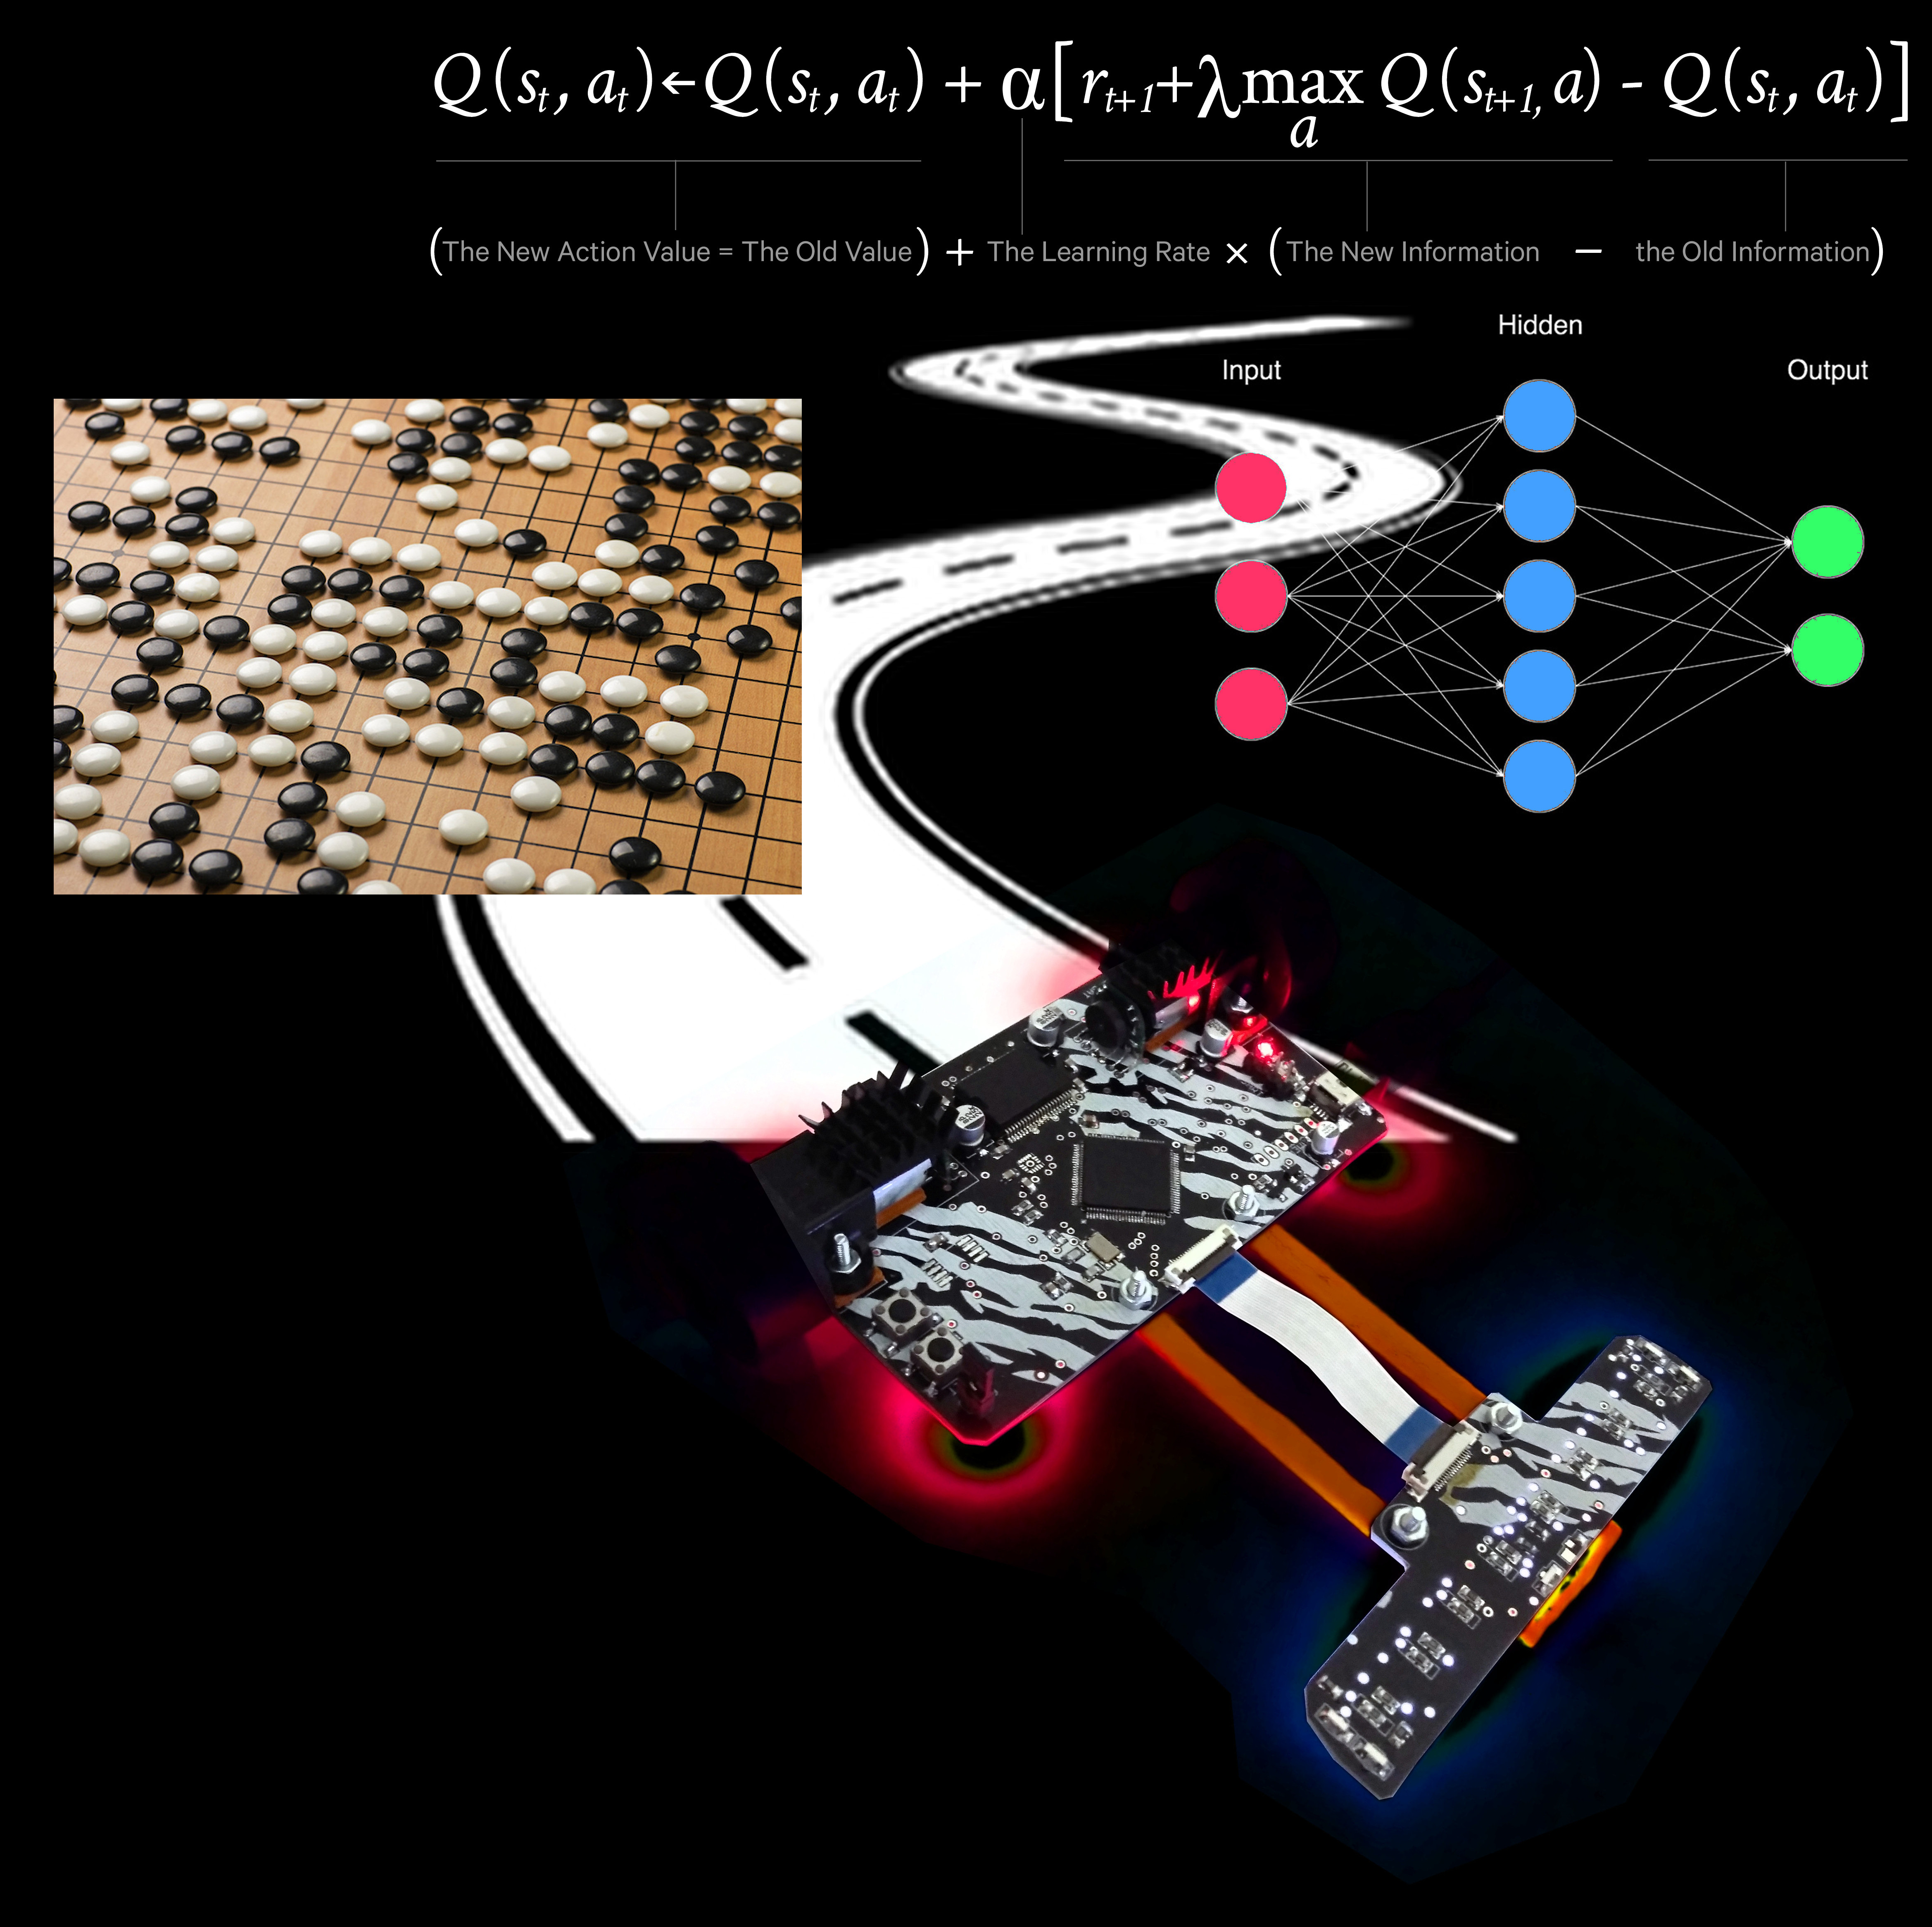
\includegraphics[width=5.05in]{./pictures/rl_square.jpg}}

        \hfil}\vfil}
    }
    \begin{frame}

    %\titlepage


    \centering
     \colorbox{black}
     {
        \begin{minipage}{7cm}
           {\LARGE \color{white} \bf reinforcement learning \\ - deep Q networks} \\
           {\LARGE \color{white} Michal CHOVANEC} \\
       \end{minipage}
     }


    \end{frame}
}

\begin{frame}{\bf reinforcement learning}

\begin{columns}
  \begin{column}{0.5\textwidth}
      \centering
      \includemovie[
        poster,
        autoplay,
        externalviewer,
        inline=false,
        text={ 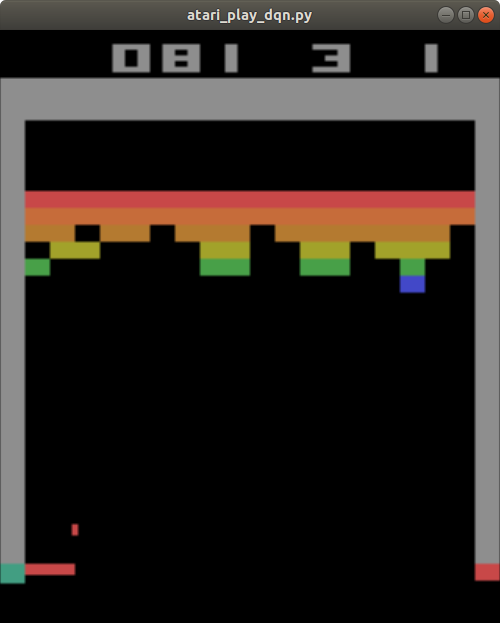
\includegraphics[scale=0.15]{./pictures/breakout.png}}
      ]{4cm}{4cm}{./video/rl_atari.mp4}

  \begin{figure}
    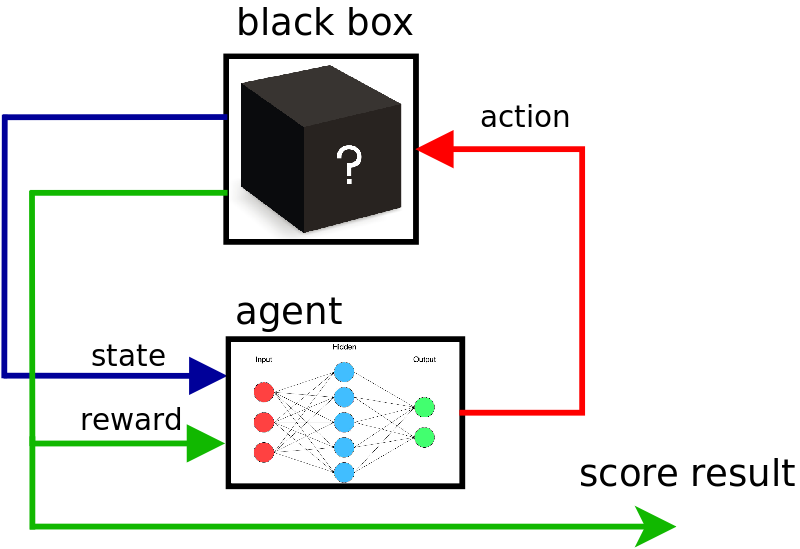
\includegraphics[scale=0.2]{./diagrams/rl_mechanism.png}
  \end{figure}

  \end{column}
  \begin{column}{0.5\textwidth}  %%<--- here

  {\bf
    \begin{itemize}
      \item learning from punishments and rewards
      \item learn to play a game with unknow rules
    \end{itemize}
  }

  \begin{enumerate}
    \item obtain {\bf state}
    \item choose {\bf action}
    \item {\bf execute} action
    \item obtain {\bf reward}
    \item learn from {\bf experiences}, $Q(s, a)$, or $\pi(a|s)$
  \end{enumerate}


  \end{column}
\end{columns}

\end{frame}


\begin{frame}{\bf Q-learning}


\begin{columns}
  \begin{column}{0.5\textwidth}
    
    $Q(s, a)$ : what is the potential reward in state {\bf s} and action {\bf a}

    \begin{align*}
      Q'(s, a) = R(s, a) + \gamma \max \limits_{a'} Q(s', a')
    \end{align*}

  \end{column}
  \begin{column}{0.5\textwidth}  %%<--- here

    where \\
    $s$ is state \\
    $a$ is action \\
    $s'$ is next state \\
    $a'$ is best action in next state \\
    $R(s, a)$ is reward \\
    $\gamma \in \langle 0, 1 \rangle$ is discount factor \\

  \end{column}
\end{columns}

\begin{figure}
  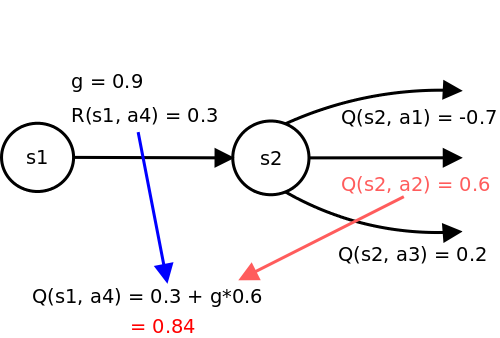
\includegraphics[scale=0.25]{diagrams/q_learning_detail.png}
\end{figure}

\end{frame}


\begin{frame}{\bf Q function}




\begin{columns}
  \begin{column}{0.5\textwidth}
    
    {\bf Q(s, a) = ?}

    \begin{itemize}
      \item table
      \item linear combination of basis functions
      \item neural network
    \end{itemize}

    {\bf number of states}
    \begin{itemize}
      \item atoms in observable universe, $10^{80}$
      \item chess, $10^{120}$
      \item go, $10^{180}$
      \item star craft, $10^{500}$
    \end{itemize}


  \end{column}
  \begin{column}{0.5\textwidth}  %%<--- here

    \begin{figure}
      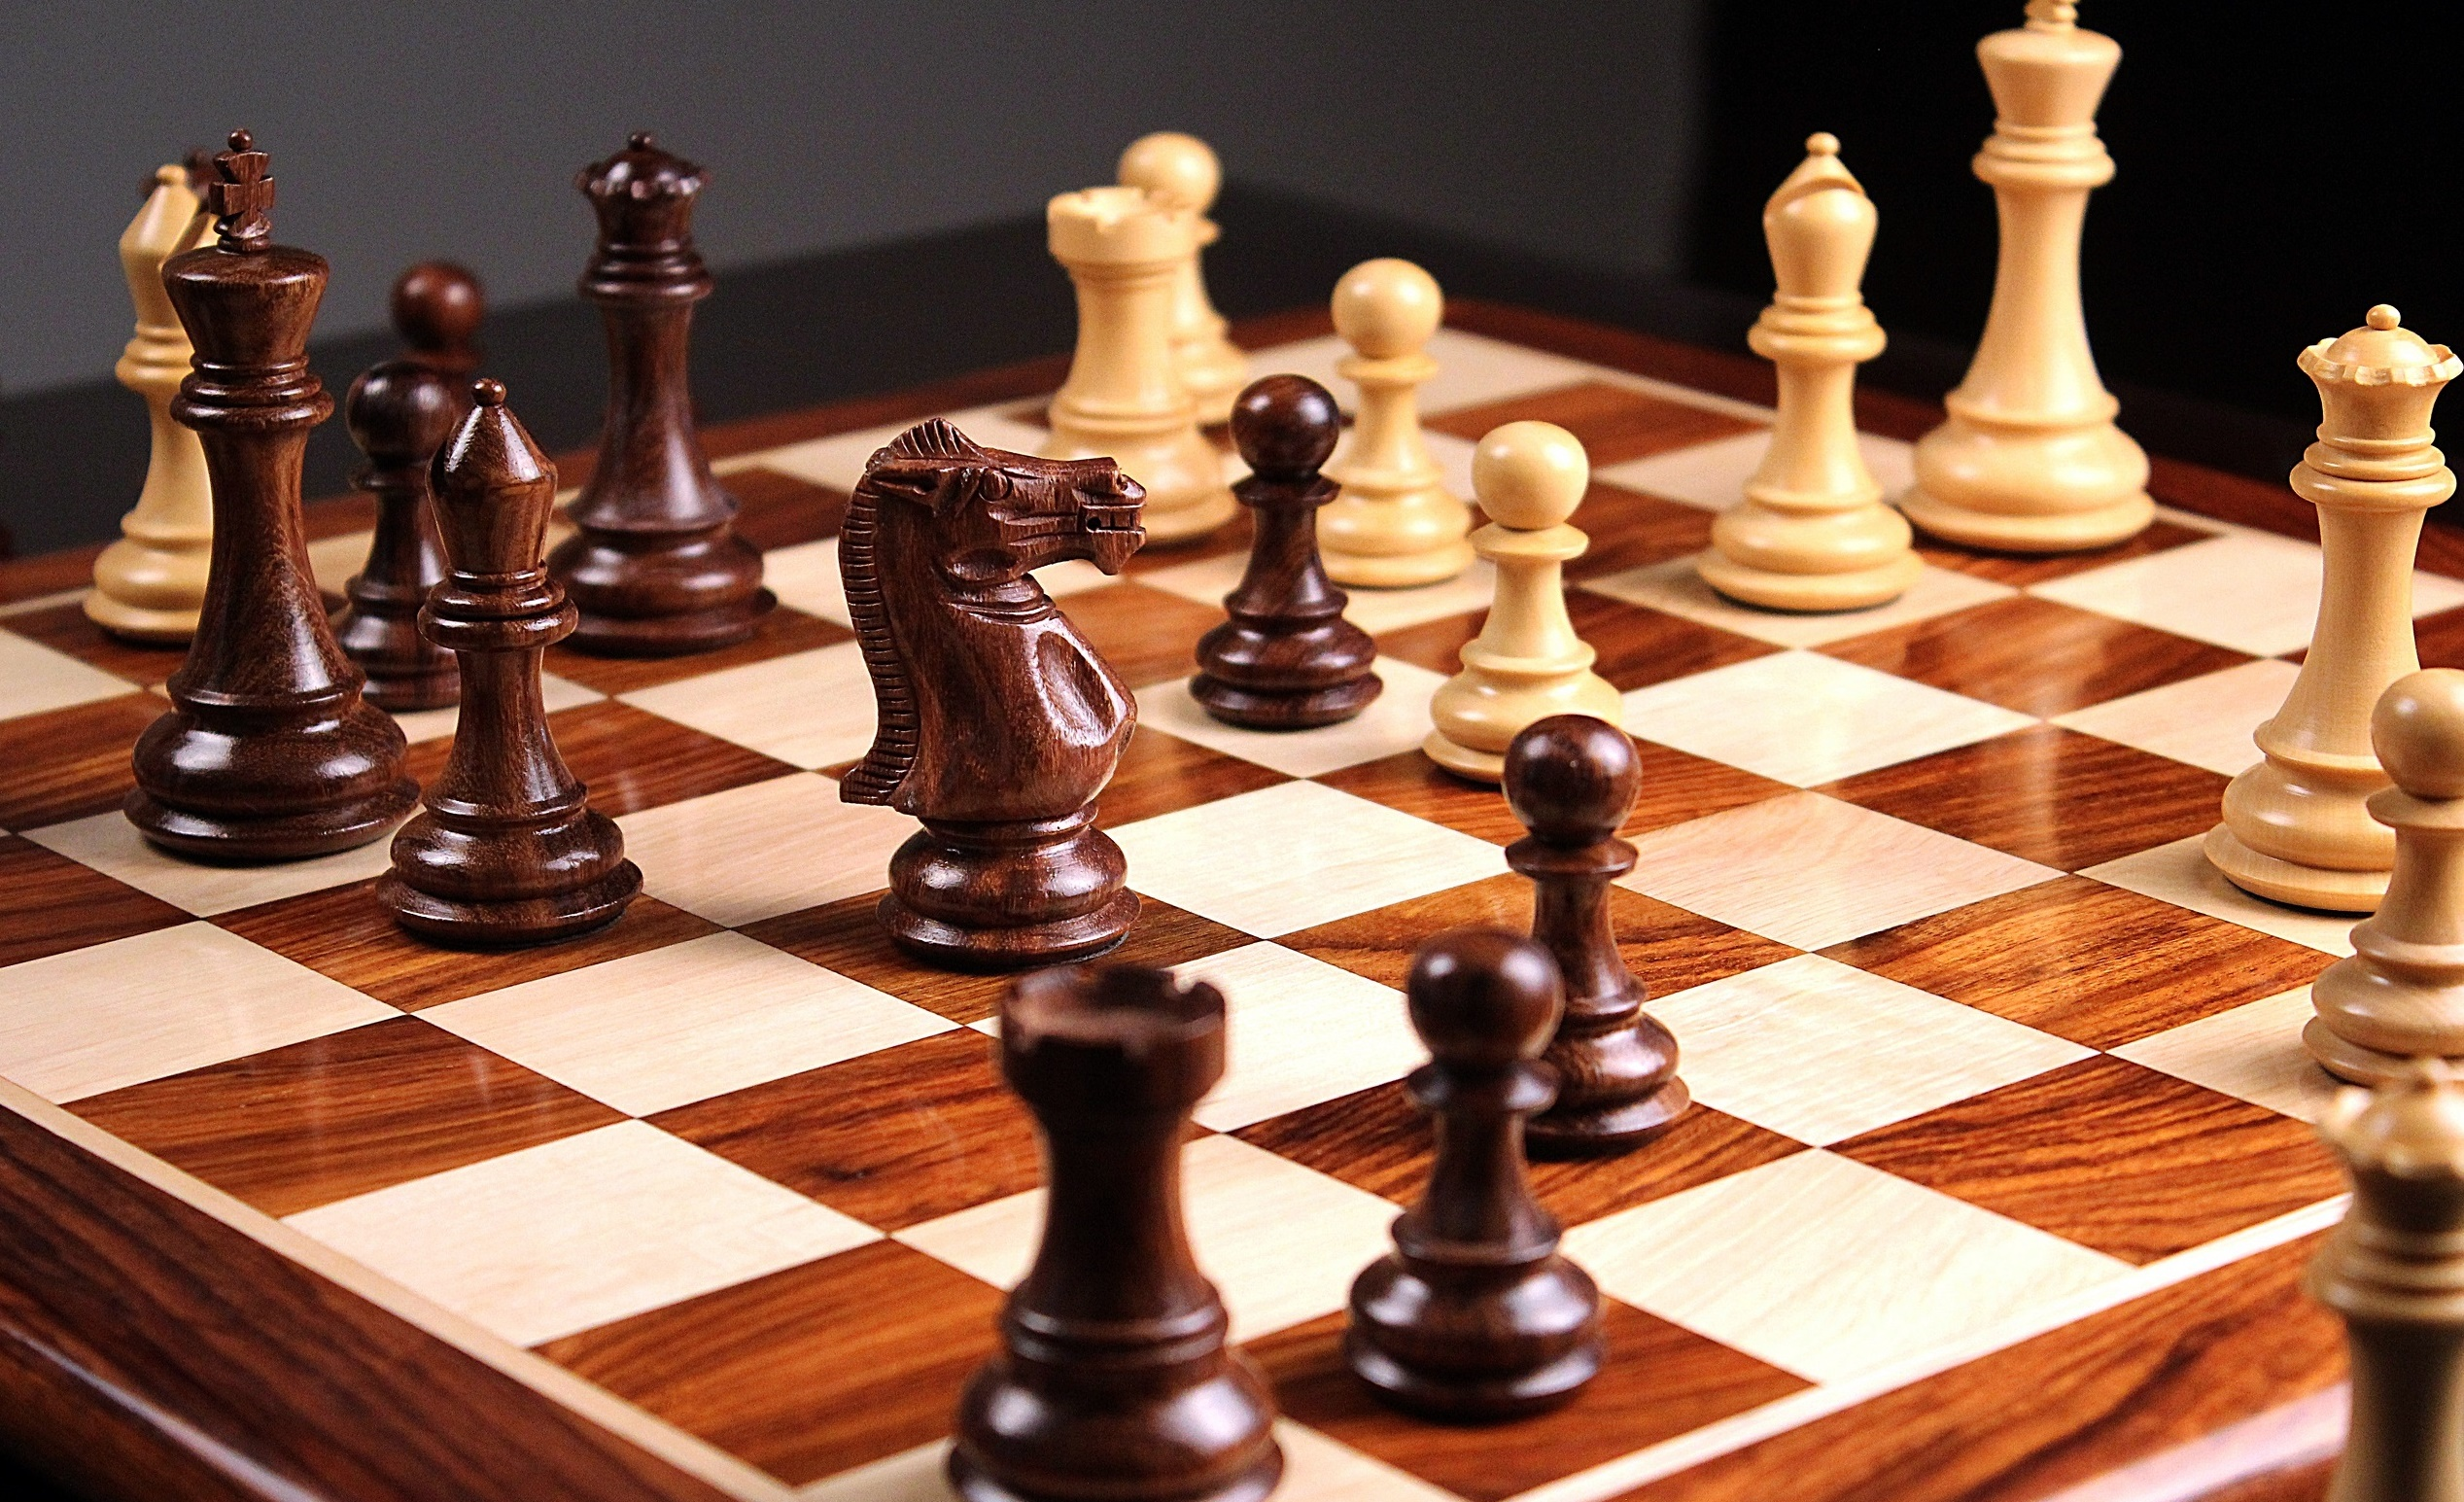
\includegraphics[scale=0.03]{pictures/chess.jpg}
    \end{figure}

    \begin{figure}
      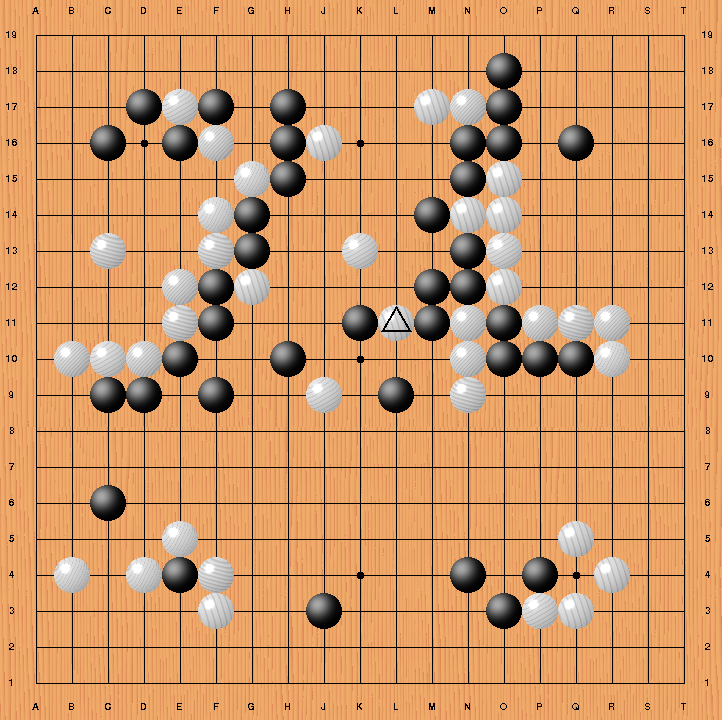
\includegraphics[scale=0.08]{pictures/alphago.png}
    \end{figure}

    \begin{figure}
      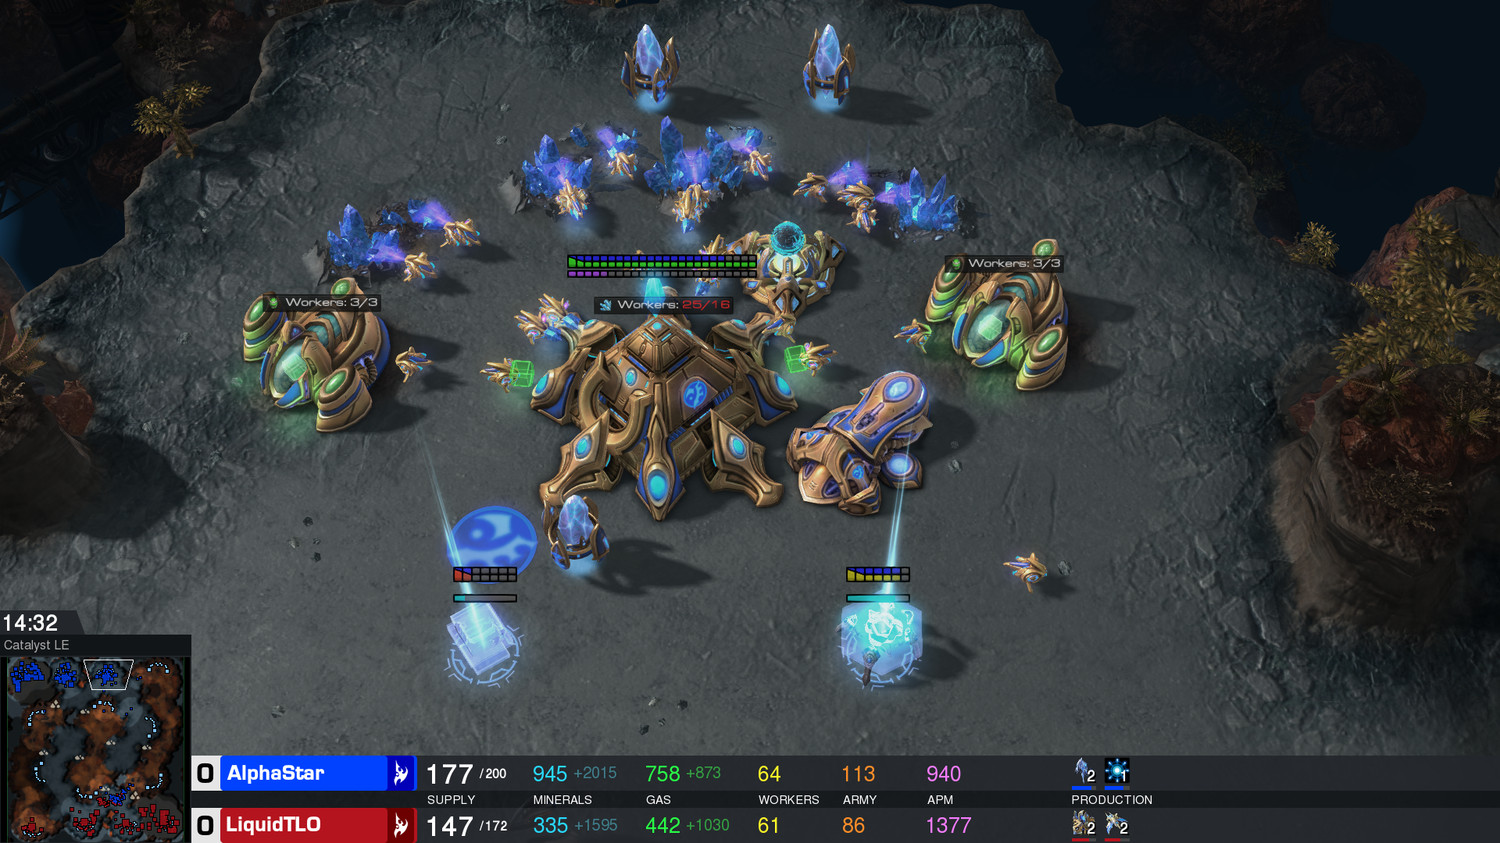
\includegraphics[scale=0.08]{pictures/alphastar.jpg}
    \end{figure}

  \end{column}
\end{columns}


\end{frame}






\begin{frame}{\bf Naive solution}

\begin{figure}
  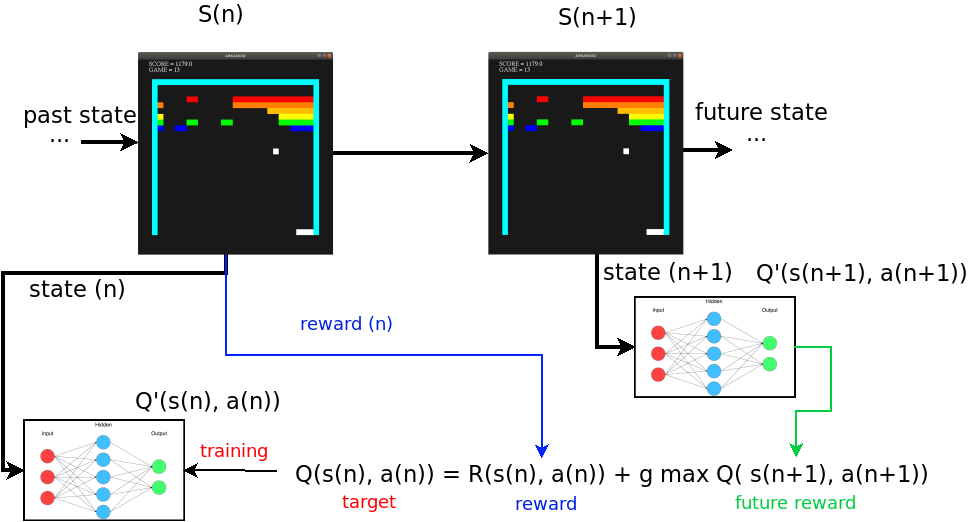
\includegraphics[scale=0.25]{./diagrams/dqn_naive.png}
\end{figure}

\end{frame}

\begin{frame}{\bf Deep Q network - DQN}

\begin{itemize}
\item {\bf \color{red} correlated states} : experience replay buffer \\
\item {\bf \color{red} unstable training} : non-stationary target value $\hat{Q}(s, a; w)$, depends on $w$, use temporary fixed weights w' \\
\item {\bf \color{red} unknow gradients values} : clip or normalise gradients and Q values
\end{itemize}
{\bf DQN equation}
\begin{align*}
  \hat{Q}(s, a; w) &= R + \gamma \max \limits_{\alpha'} \hat{Q}(s', \alpha'; w') \\
  \mathcal{L}(w) &= (R + \gamma \max \limits_{\alpha'} \hat{Q}(s', \alpha'; w') - \hat{Q}(s, a; w))^2
  \label{eq:dqn}
\end{align*}

%E &= R + \gamma \max \limits_{\alpha'} \hat{Q}(s', \alpha'; w') - \hat{Q}(s, a; w)


\begin{figure}[!htb]
  \centering
  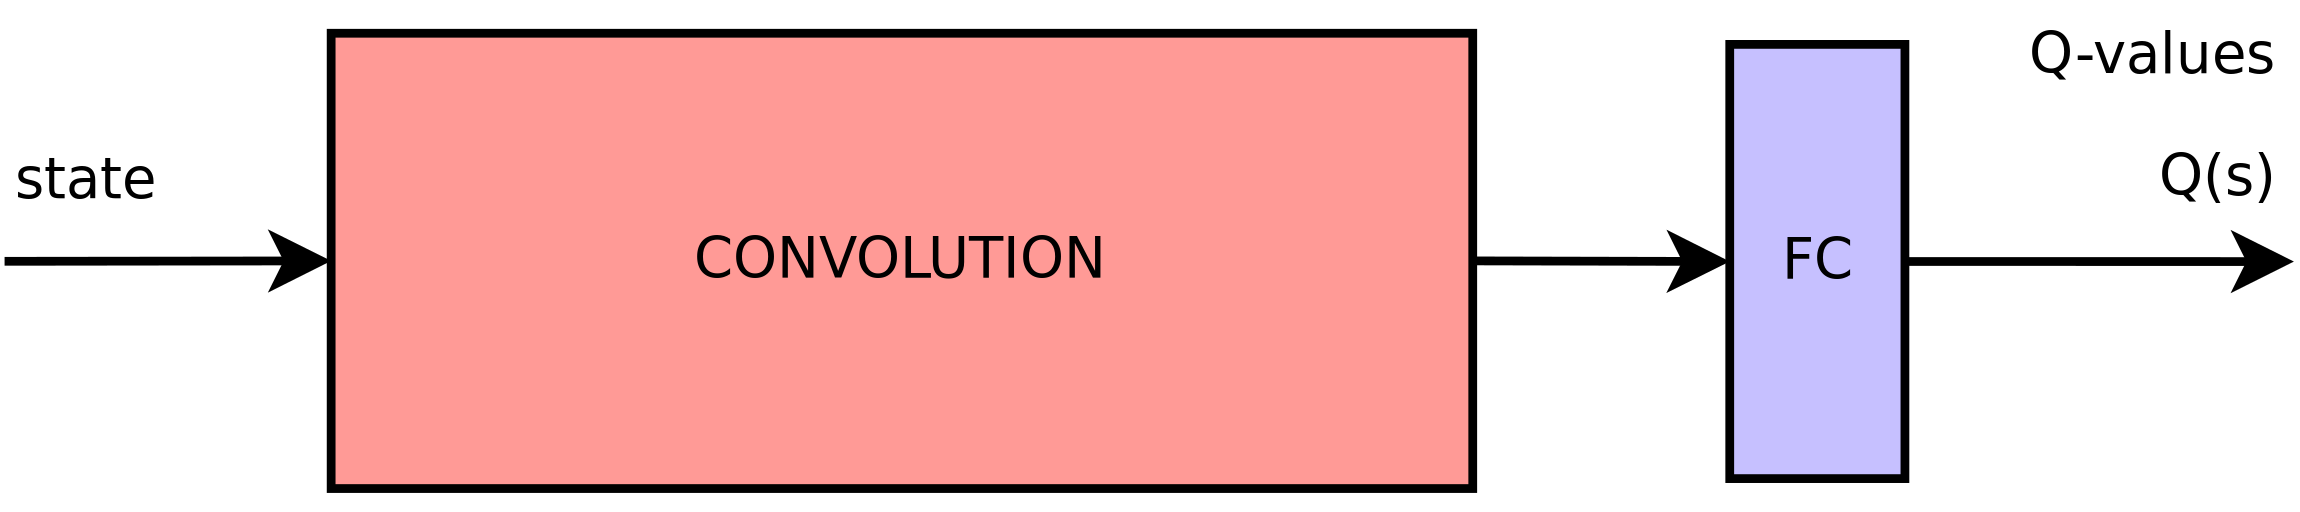
\includegraphics[scale=0.16]{./diagrams/dqn.png}
  \label{img:dqn}
\end{figure}


\end{frame}





















\begin{frame}{\bf deep Q network - DQN}

$Q(s, a)$ : what is the potential reward in state $s$ and action $a$

\begin{figure}
  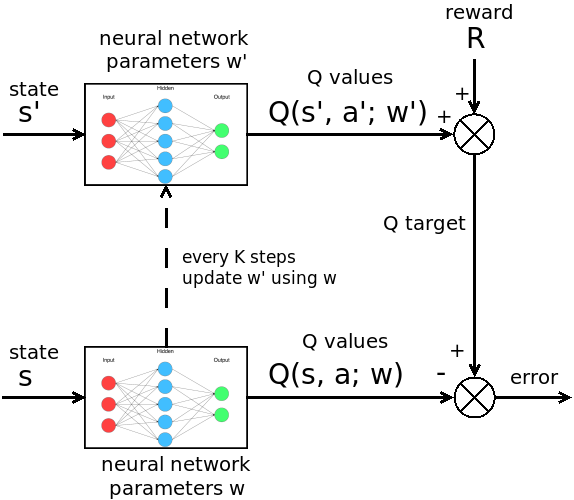
\includegraphics[scale=0.3]{./diagrams/dqn_detail.png}
\end{figure}

\begin{align*}
\mathcal{L}= &\left( \underset{\bf \color{green} target\ value}{ R + \gamma \max \limits_{\alpha'} Q(s', \alpha'; w') } - \underset{\bf \color{red} predicted\ value}{Q(s, a; w)} \right) ^2
\end{align*}

\end{frame}


\begin{frame}{\bf be more specific}
\begin{itemize}
  \item state  : \begin{itemize}
                  \item  grayscale frames, 
                  \item size 96x96, (84x84) 4 past frames - frame stacking
                  \item use wrappers (life lost reward, frame skipping, reset fire button)
                \end{itemize}
  \item reward : clip into range $\langle -1, 1 \rangle$
  \item discount factor $\gamma = 0.99$
  \item update rate $k = 4$
\end{itemize}


\begin{figure}
  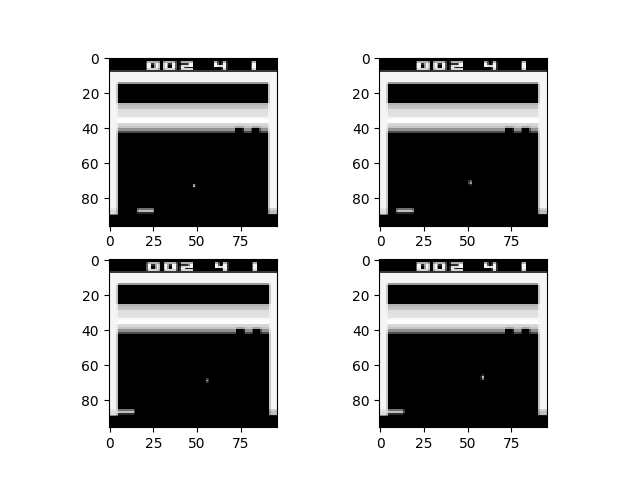
\includegraphics[scale=0.4]{./pictures/breakout_state.png}
\end{figure}

\end{frame}






\end{document}
